\iffalse
\let\negmedspace\undefined
\let\negthickspace\undefined
\documentclass[journal,12pt,twocolumn]{IEEEtran}
\usepackage{cite}
\usepackage{amsmath,amssymb,amsfonts,amsthm}
\usepackage{algorithmic}
\usepackage{graphicx}
\usepackage{textcomp}
\usepackage{xcolor}
\usepackage{txfonts}
\usepackage{listings}
\usepackage{enumitem}
\usepackage{mathtools}
\usepackage{gensymb}
\usepackage{comment}
\usepackage[breaklinks=true]{hyperref}
\usepackage{tkz-euclide} 
\usepackage{listings}
\usepackage{gvv}                                        
\def\inputGnumericTable{}                                 
\usepackage[latin1]{inputenc}                                
\usepackage{color}                                            
\usepackage{array}                                            
\usepackage{longtable}                                       
\usepackage{calc}                                             
\usepackage{multirow}                                         
\usepackage{hhline}                                           
\usepackage{ifthen}                                           
\usepackage{lscape}
\usepackage{amsmath}
\usepackage{caption}

\newtheorem{theorem}{Theorem}[section]
\newtheorem{problem}{Problem}
\newtheorem{proposition}{Proposition}[section]
\newtheorem{lemma}{Lemma}[section]
\newtheorem{corollary}[theorem]{Corollary}
\newtheorem{example}{Example}[section]
\newtheorem{definition}[problem]{Definition}
\newcommand{\BEQA}{\begin{eqnarray}}
\newcommand{\EEQA}{\end{eqnarray}}
\newcommand{\define}{\stackrel{\triangle}{=}}
\theoremstyle{remark}
\newtheorem{rem}{Remark}
\begin{document}

\bibliographystyle{IEEEtran}
\vspace{3cm}

\title{GATE: CH-62 2023}
\author{EE23BTECH11038 - Rohith Madhani$^{*}$% <-this % stops a space
}
\maketitle
\newpage
\bigskip
\renewcommand{\thefigure}{\theenumi}
\renewcommand{\thetable}{\theenumi}

\textbf{Question :} The transfer function of a measuring instrument is \\
$$G_m(s) = \frac{1.05}{2s+1}exp(-s)$$
At time $t = 0$, a step change of +1 unit is introduced in the input of this instrument.The time taken by the instrument to show an increase of 1 unit in its output is(rounded off to two decimal places). \\ \hfill(GATE CH 2023) \\
\solution
\fi

\begin{table}[!h] 
\centering
\begin{table}[ht]
	  \centering
	    \begin{tabular}{|c|c|c|}
		        \hline
			   \textbf{ Parameter} & \textbf{Value} & \textbf{Description} \\
			       \hline
			           $v\brak{t}$ & $100cos\brak{\omega_0 t}$ & Input Voltage \\
				       \hline
				           $R$ & $1\text{ k}\Omega$ & Resistance \\
					       \hline
					           $C$ & $100\mu\text{F}$ & Capacitance \\
						       \hline
						           $\omega_0$ & ? & Angular Frequency  \\
							       \hline
							           $Z_R = R$ & $10^3$ & Impedance for resistor  \\
								       \hline
								           $Z_C = \frac{1}{j\omega C}$ & $\frac{10^{4}}{j\omega_0}$ & Impedance for capacitor  \\
									       \hline
									           $Z = R + \frac{1}{j\omega C}$ & $10^3 + \frac{10^4}{j\omega_0}$ & Total Impedance \\
										       \hline
										         \end{tabular}
											   \vspace{2mm}
											     \caption{Parameter Table}
											       \label{BM_23_32}
\end{table}

\caption{Given parameters}
\label{table:gate23ch62}
\end{table}

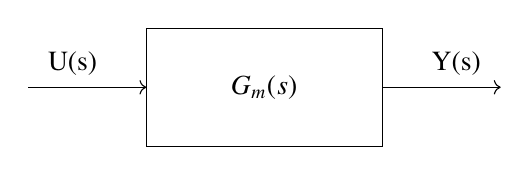
\begin{tikzpicture}
\centering
    % Draw the main box
    \node[draw, minimum width=3cm, minimum height=1.5cm] (box) at (0,0) {$G_m(s)$};
    
    % Draw the input arrow
    \draw[->] (-3,0) -- (-1.5,0);
    
    % Draw the output arrow
    \draw[->] (1.5,0) -- (3,0);
    
    % Label the input arrow
    \node[anchor=east] at (-2,0.3) {U(s)};
    
    % Label the output arrow
    \node[anchor=west] at (2,0.3) {Y(s)};
\end{tikzpicture}

\begin{align}
    G_m(s) &= \frac{1.05}{2s+1}e^{-s} \\
    \because Y(s) &= G_m(s).U(s) \\
    \implies Y(s) &= \frac{1}{s}.\frac{1.05}{2s+1}e^{-s}
\end{align}

By splitting into partial fractions,we get
\begin{align}
    Y(s) &= \sbrak{\frac{1.05}{s} - \frac{1.05}{s+0.5}}e^{-s}
\end{align}

As we know,
\begin{align}
    \mathcal{L}[e^{-at}] &\system{} \frac{1}{s+a} \\
    \mathcal{L}[f(t-1)] &\system{} e^{-s}F(s)
\end{align}

By taking inverse laplce we get,

\begin{align}
    y(t) &= 1.05\sbrak{1-e^{\frac{-(t-1)}{2}}}u(t-1) \\
    \frac{1}{1.05} &= 1-e^{\frac{-(t-1)}{2}} \\
    \frac{-(t-1)}{2} &= \ln(\frac{0.05}{1.05}) \\
    \implies t &= 7.073 
\end{align}

\begin{figure}[h]
    \centering
    \includegraphics[width=\columnwidth]{2023/CH/62/figs/fig1.png}
    \caption{y(t) = $1.05\sbrak{1-e^{\frac{t-1}{2}}}$}
    \label{fig:gate23ch62}
\end{figure}

%\end{document}
